\documentclass[compress,xcolor={dvipsnames}]{beamer}
\usepackage{fancyvrb,newverbs} % For customized verbatim
\usepackage{calligra} % A fancy text for ending `Thank you'
\usepackage[T1]{fontenc}
\usepackage{outline}
\usepackage{changepage}
\usepackage{animate}
\usefonttheme[onlymath]{serif}

\author{Zihang Wang}
\title{Phase Field Tutorial}
\subtitle{Phase Field Simulation of Grain Growth}
\institute{Central South University}

\AtBeginSubsection[]
{
	\begin{frame}
		\tableofcontents[sectionstyle=show/shaded,subsectionstyle=show/shaded/hide,subsubsectionstyle=show/shaded/hide]
	\end{frame}
}
\usetheme{Berlin} 

\setbeamertemplate{footline} {
    \begin{beamercolorbox}[ht=2.5ex,dp=1.125ex,
      leftskip=.3cm,rightskip=.3cm plus1fil]{title in head/foot}
      {\usebeamerfont{institute in head/foot}\usebeamercolor[fg]{institute in head/foot}\insertshortinstitute}
      \hfill
      {\centering\usebeamerfont{title in head/foot}\insertshortsubtitle}
      \hfill
      {\usebeamerfont{frame number}\usebeamercolor[fg]{frame number}\insertframenumber~/~\inserttotalframenumber}
    \end{beamercolorbox}
    \begin{beamercolorbox}[colsep=1.5pt]{lower separation line foot}
    \end{beamercolorbox}
}

% ---------------------------------------------------------------------------
\definecolor{cverbbg}{gray}{0.93}

\newenvironment{cverbatim}
 {\SaveVerbatim{cverb}}
 {\endSaveVerbatim
  \flushleft\fboxrule=0pt\fboxsep=.5em
  \colorbox{cverbbg}{\BUseVerbatim{cverb}}%
  \endflushleft
}
\newenvironment{lcverbatim}
 {\SaveVerbatim{cverb}}
 {\endSaveVerbatim
  \flushleft\fboxrule=0pt\fboxsep=.5em
  \colorbox{cverbbg}{%
    \makebox[\dimexpr\linewidth-2\fboxsep][l]{\BUseVerbatim{cverb}}%
  }
  \endflushleft
}
\newverbcommand{\cverb}
  {\setbox\verbbox\hbox\bgroup}
  {\egroup\colorbox{cverbbg}{\box\verbbox}}

\setlength{\parindent}{2em}

\newcommand{\bhref}[2]{
    \href{#1}{\color{blue}{#2}}
}
% ---------------------------------------------------------------------------

\begin{document}
\begin{frame}
    \titlepage
    \begin{figure}[!h]
        \centering
        
\includegraphics[width=0.18\linewidth]{pic/csulogo.jpg}
        
\includegraphics[width=0.25\linewidth]{pic/MInDes_Icon.jpg}
    \end{figure}
\end{frame}

\begin{frame}
    \tableofcontents[currentsection, hideothersubsections, sectionstyle=show/show]
\end{frame}

% ---------------------------------------------------------------------------
\section{Review \& Intro}
\begin{frame}
    \frametitle{Quick Review}
    In last tutorial, we learned about spinodal decomposition, and went through the phase field simulation of this phase transformation process. Here's a quick review.

    \begin{itemize}
        \item Spinodal Decomposition Introduction
        \item Simulation Code Structure
        \item Implementation
        \item Result Visualization
    \end{itemize}

    In this tutorial, we are going to use the phase field method to simulate the grain growth process, which is another good example of the Allen-Cahn equation.

\end{frame}

\subsection{Grain Growth Process}
\begin{frame}
    \frametitle{Grain Growth}

    We are already familiar with the concepts of grain growth. After nucleation of grain from liquid or solid phase, the nuclei will growth due to the grain growth driving force, which is a combination of body free energy and grain boundary free energy. With the grain growth, the former one will increase and the later one will decrease, due to the increament of grain size and decreament of boundary length. Here is a 3D simulation result of grain growth process: \bhref{pic/Grgr3d_small.gif}{3D Grain Growth}.

\end{frame}

\subsection{Phase Field Model}
\begin{frame}
    \frametitle{Free Energy Construction}

    Let's have a look at the energy construction we are going to use for grain growth process:
    \[
        F = \int_\omega f_b + \sum_{i}^{N}\frac{\kappa_i}{2} \left( \nabla \eta \right)^2 \,\mathrm{d}\Omega.
    \]
    It looks very similar to the energy construction we haven seen before, with a little difference if we don't care about the exact bulk energy form. The boundary contribution here is not just a single term gonverned by `concentration', but a sum of square of \emph{field variable} or \emph{order parameter}. Here, \(N\) means that we have N-grains The order parameter acts like concentration, but the sum of order paramter could be any value instead of just be a fixed finite value. That's so-called \emph{non-conservative parameter}. We shall come back to this latter.

\end{frame}

\begin{frame}
    \frametitle{Bulk Energy Form}

    Now let's shed some light on the bulk energy. For this simulation, we adopt the model from the work of Fan and Chen\footnote{Fan D, Chen LQ (1997) Computer simulation of grain growth using a continuum field model. Acta Mater 45:611}:\vspace{-7pt}
    \[
        f_b(\eta_0,\eta_1, \cdots, \eta_N) = \sum_{i}^{N}\left( -\frac{A}{2}\eta_i^2 + \frac{B}{4}\eta_i^4 \right) + \sum_{i}^{N}\sum_{j\neq{}i}^{N}\eta_i^2\eta_j^2
    \]
    \vspace{-7pt}

    Before having a visualization of this function, we can analyse this function mathematically first. Let's look at the first sum: this is actually a double well shape with lowest point locates at -1 and 1. While, we are only going to take the positive part though. Then we can view the second double-sum as a coefficient of \(\eta_i^2\), whereas the coefficient describes the influence of other phases (grains).

\end{frame}

\begin{frame}
    \frametitle{Bulk Energy Curve}
    Consider at one point in the simulation field. This points locates either in the grain or the grain boundary. If it's in the grain, then order parameter of this grain should be 1, and any other order parameter should be zero. This matches the function well; If this point is in the grain boundary, then there will be many order parameters be non-zero, and the potential well position for each grain will be shifted far from 1, indicates that there is a boundary.

    \begin{columns}
        \begin{column}{.5\linewidth}
            You are welcomed to using tools like \bhref{https://www.desmos.com/calculator?lang=zh-CN}{Desmos} to visualize this function. And on the right side there is a 3D plot of this function of two phase presented with \(A=B=1\):
        \end{column}
        \begin{column}{.4\linewidth}
            \begin{figure}
                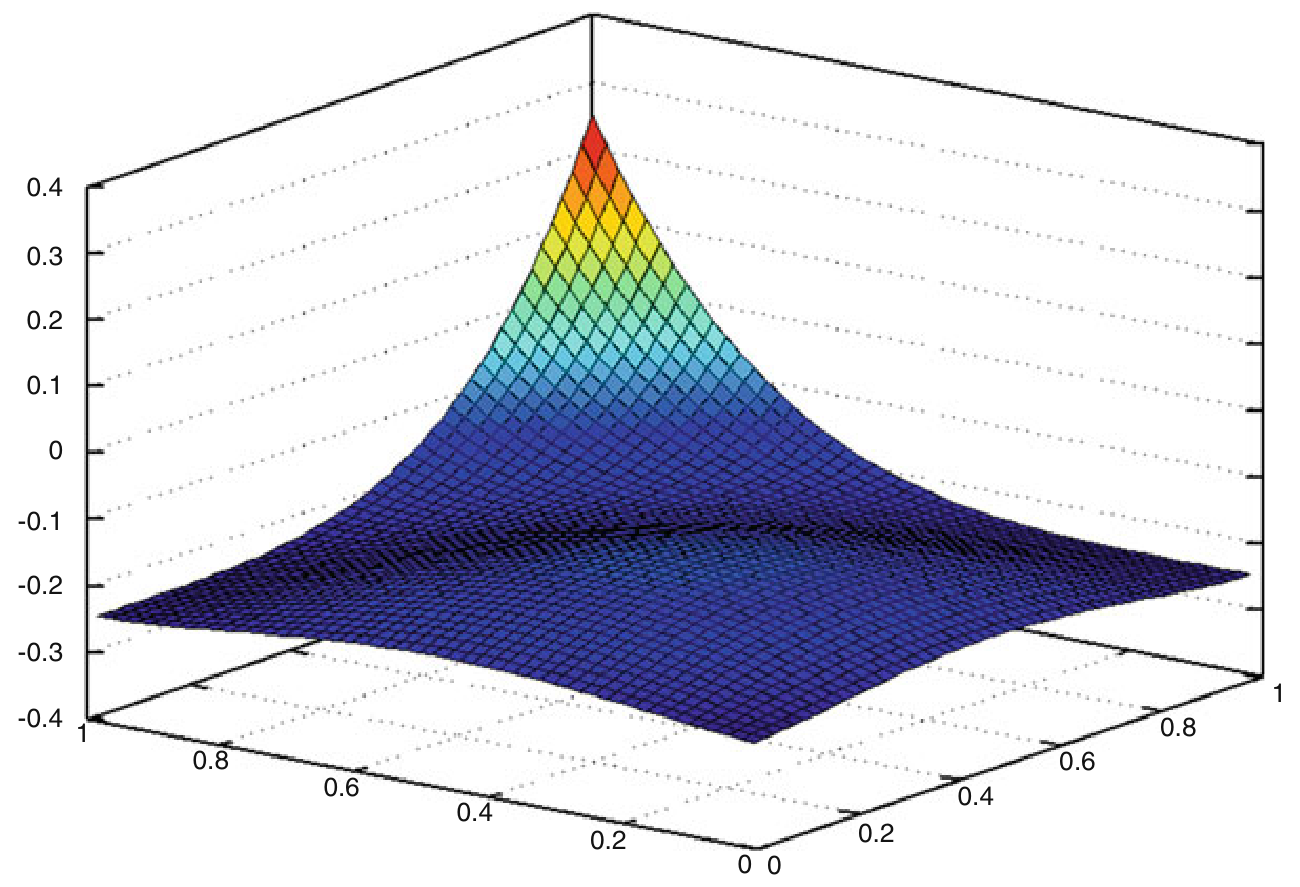
\includegraphics[width=\linewidth]{pic/bulk_energy.png}
            \end{figure}
        \end{column}
    \end{columns}


\end{frame}

\begin{frame}
    \frametitle{Allen-Cahn Equation}

    We mentioned before that the order parameter we considered here is non-conservative. To deal with non-conservative order parameter, we should use so-called \emph{Allen-Cahn Equation}:
    \[
        \frac{\partial \eta_i}{\partial t} = -L_i \frac{\delta F }{\delta \eta_i },
    \]
    where \(i\) takes from 1 to \(N\). The basic idea behind this equation is rather simple. When a system is balanced, then the variation of free energy with respect to each parameter (which is indeed driving force if parameter is not time or space) should be 0. If the system is not balanced, then the variable's evolution direction must be the one decreasing the driving force. Hence, the most simple form to express this relation shall be this equation.

\end{frame}

\subsection{Today's Target}
\begin{frame}
    \frametitle{Grain Growth}

    There are actually may simulation we can do for grain growth. What we are going to do is simulate the double grain growth process. Like what we have already done in the last tutorial, we will:
    \begin{itemize}
        \item Analyse the question and prepare for the simulation
        \item Write C++ program to carry out the simulation of grain growth
        \item Analyse the simulation result
    \end{itemize}

    And as usual, we are going to list the parameters and equations we are going to use, give a brief code structure, and finally implement the code from the scratch.
\end{frame}

\section{Simulation}
\subsection{Preparation}
\begin{frame}[fragile]
    \frametitle{Parameter List}
    \begin{center}

        \begin{tabular}{ccc}
            \hline
            Parameters                          & Value    & Type           \\
            \hline
            \(N_x\) \& \(N_y\)                  & 64       & \cverb|int|    \\
            \(\mathrm{d}x\) \& \(\mathrm{d}y\)  & 0.5      & \cverb|double| \\
            \(\mathrm{d}t\)                     & 0.005    & \cverb|double| \\
            simulation step (\cverb|nstep|)     & 20000    & \cverb|int|    \\
            output step (\cverb|pstep|)         & 100      & \cverb|int|    \\
            initial grain size (\cverb|radius|) & 14       & \cverb|int|    \\
            mobility \(L_i\) (\cverb|mobility|) & 5.0      & \cverb|double| \\
            gradient coefficient \(\kappa\)     & 0.1      & \cverb|double| \\
            free energy parameter \(A,\,B\)     & 1.0      & \cverb|double| \\
            boundary condition                  & periodic & -              \\
            boundary value truncate             & 1e-6     & \cverb|double| \\
            \hline
        \end{tabular}

    \end{center}

\end{frame}

\begin{frame}
    \frametitle{Formulae to Use}

    Time iterate:
    \[
        \textstyle
        \eta_{i}^{n+1} = \eta^n_{i}- \Delta t  L \left( \frac{\delta F}{\delta \eta_{i}} \right)^n;
    \]
    Energy variation:
    \[
        \textstyle
        \left( \frac{\delta F}{\delta \eta_i} \right)^n = \mu\left(\eta^n_{i}\right) - \kappa\nabla^2\eta^n_{i};
    \]
    Chemical potential:
    \begin{align*}
        \textstyle \mu(\eta_i^n) & \textstyle =  -A\eta_i^n+B(\eta_i^n)^3+2\eta_i^n\sum_{j\ne{}i}^{N}(\eta_j^n)^2;                                     \\
                                 & \textstyle = -A \eta_i^n+B(\eta_i^n)^3+2\eta_i^n\left( \sum_{j}^{N}\left( \eta_j^n \right)^2 - (\eta_i^n)^2 \right)
    \end{align*}
\end{frame}

\begin{frame}[fragile]
    \frametitle{Code Structure}

    Here the code structure to accomplish the simulation is presented as follows:
    \begin{columns}
        \begin{column}{.5\linewidth}
            \begin{itemize}
                \item Headers
                \item Tool Functions
                      \begin{itemize}
                          \item Free energy derivative
                          \item Laplacian calculation
                          \item Data output
                      \end{itemize}
            \end{itemize}
        \end{column}
        \hspace{-20pt}
        \begin{column}{.5\linewidth}
            \begin{itemize}
                \item \cverb|main| function
                      \begin{itemize}
                          \item Constants
                          \item Mesh initialization
                          \item Time step loop
                          \item Phase loop 1
                          \item Mesh loop 1
                          \item Phase loop 2
                          \item Mesh loop 2
                          \item Data output
                      \end{itemize}
            \end{itemize}
        \end{column}
    \end{columns}

\end{frame}

\subsection{Code Implementation}
\begin{frame}
    \frametitle{Write It Now}

    Now let's write this simulation by hand from scratch.

    The completed code will be avaliable after this tutorial. There will be more example on this tutorial, such as OOP Implementation, algorithm optimization, voronoi structure generation and simulation, and so on, in the future. You can check them with my \bhref{https://github.com/A-moment096/Phase-Field-Tutorial}{Github}

\end{frame}
\subsection{Results}
\begin{frame}
    \frametitle{Visualization}

    We choose Paraview to open the data files we generated from the program, which are \emph{vtk} files.

\end{frame}

\section{Summary}
\begin{frame}
    \frametitle{Exercise}

    Below are some exercises for today's contents, basically the same as the last tutorial:

    \begin{enumerate}
        \item Please try to write today's code and run it by yourself.
        \item Modify the parameters related to the free energy and governing equation, for example, the gradient coefficient \(\kappa\) and analyse the results.
        \item Modify the parameters related to the calculation, for example, \(\mathrm{d}x\) or \(\mathrm{d}t\), and analyse the results. Please be careful when adjust them as these parameters might influence the stability of the calculation.
    \end{enumerate}

    Besides these exercises, you are encouraged to try modifying the simulation model by yourself to see the influence.

\end{frame}

\begin{frame}
    \frametitle{Resources}

    Here are some resources that might help you.
    \begin{itemize}
        \item Today's contents are mainly from the book we have been always refered to, \emph{Programming Phase Field Modeling}. You will find matlab\textsuperscript{\textregistered} code in this book about today's simulation. You are welcomed to translate the matlab\textsuperscript{\textregistered} code into C++ or other programming language.
        \item For the result visualization, \emph{vtk} file format is used. For more information about this file format, you can refer to \bhref{https://docs.vtk.org/en/latest/design_documents/VTKFileFormats.html}{VTK file format reference}.
    \end{itemize}
\end{frame}

\begin{frame}
    \frametitle{Summary}

    So this is the second example of phase field simulation. By now, we have already seen the two very basic gonverning equations, the Cahn-Hilliard equation and Allen-Cahn equation, about when and how they are used with a set of tools, mathematical or computational, to carry out a phase field simulation.

    Of course there are more about this tutorial, such as grain growth can be more complex in terms of free energy construction, choosing different gonverning equations instead of basic Allen-Cahn equation such as multi-phase field model from Ingo Steinbach, and you can even optimize the code itself, about the algorithm, computational complexity, parallel programming and so on. Please feel free to explore them.

\end{frame}

\begin{frame}
    \frametitle{Summary}

    Also, this is the last part of this series of phase field tutorials. These tutorials are only iceberg of phase field method, but I believe that the foundation of phase field simulation will never leave what we have introduced here too far. I personally sincerely hope that you got something useful during this journey of phase field learning. It's my great honour if you found things in these tutorials are useful, no matter it is mathematical part, programming part (which, personally I like most), or the simulation part.

    Finally, thank you for joining this journey with me. Wish you all the best!

\end{frame}

\begin{frame}
    \begin{center}
        {\Huge \calligra Thank You!}
    \end{center}
\end{frame}

\end{document}

